
\documentclass[journal,12pt,twocolumn]{IEEEtran}
\usepackage{graphicx}
\graphicspath{{./figs/}}{}
\title{
Matrix-Lines
}
\author{Kukunuri Sampath Govardhan}
\begin{document}
\maketitle
\tableofcontents
\begin{abstract}
This document shows how to find equation of a line passing trough a point (2,2) and cutting off intercepts on the axes whose sum is 9 using python.
\end{abstract}
\section{Problem Statement}
Find equation of a line passing trough a point (2,2) and cutting off intercepts on the axes whose sum is 9.\\
\section{Construction}
\begin{figure}[h]
    \centering
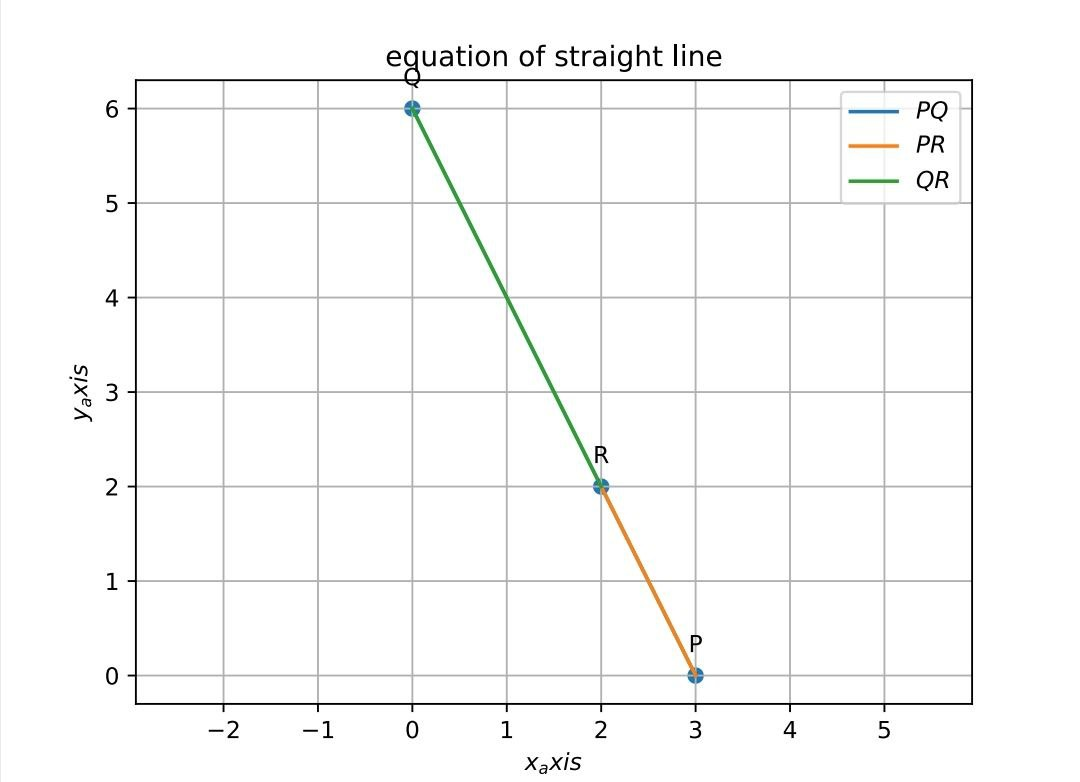
\includegraphics[width=\columnwidth]{figs/assign4.png}
    \caption{Equation of the Straight Line}
    \label{fig:my_label}
\end{figure}


    
\begin{table}[h]
    \centering
    \begin{tabular}{|c|c|c|}
       \hline
       \textbf{Symbol}&\textbf{Value}&\textbf{Description}  \\
       \hline
        P & (A,0) & Point on X-axis\\
        \hline
        Q & (0,B) & Point on Y-axis\\
        \hline
        R & (2,2) & Given Point \\
        \hline
        A+B & 9 & Given Condition\\
        \hline
    \end{tabular}
    \caption{Parameters}
    \label{tab:my_label}
\end{table}


\section{Solution}
Given that resultant line passes through point(2,2) and intercepts on axes whose sum is 9 (let x intercept is P (A,0) and y intercept is Q (0,B) therefore, A+B=9 ) so, B=9-A  \\
\\
Let P=(A,0),Q=(0,9-A),R=(2,2)\\
\\
Now we have 3 points which lies on same line so we need to find the value of A,B to find equation of the line so we find the value of p using slope(PR)=slope(RQ)\\
\\
Threrfore, we get A**2-A*p+18=0 . Using np.roots() from Numpy we get the Value of A and using this we get points A,B\\
\\
With the roots of A we find A,B respectively now we have points P,Q,R we find equation of the line using points P(x1,y1),Q(x2,y2)\\
\\
The Resultant Equation is -6x-3y+18=0 \\
\\
\section{Conclusion}
We found the equation of a line passing trough a point
(2,2) and cutting off intercepts on the axes whose
sum is 9.

\end{document}
